\usepackage[authoryear,round]{natbib}
\usepackage{multirow}

\newcommand{\sheetnum}{%
	13
}
%\setcounter{section}{\sheetnum-3}
\newcommand{\tutorialtitle}{%
    Effiicent inference in Bayesian Networks via:
    Junction Trees  \&
    Message Passing
}
\newcommand{\tutorialtitleshort}{%
    Junction Trees  \&
    Message Passing
}
% for slides
\subtitle{\sheetnum \tutorialtitle}

\maxdeadcycles=1000 % Workaround for ! Output loop---100 consecutive dead cycles because of too many figures

% The following use of algroithms does not work well with the notes:
%
%
%
%
% instead use the following for your algorithms:
%
%\begin{figure}[!t]
%\removelatexerror
%\begin{algorithm}[H]
    % your algo here
    %\label{alg:algolabel}
    %\caption{algocaption}
%\end{algorithm}
%\end{figure}
%\begin{algorithm}
% Below is the definition for the command \removelatexerror:
\makeatletter
\newcommand{\removelatexerror}{\let\@latex@error\@gobble}
\makeatother

\begin{document} %%%%%%%%%%%%%%%%%%%%%%%%%%%%%%%%%%%%%%%%%%%%%%%%%%%%%%%

\sheet{\sheetnum}{\tutorialtitleshort}

\ttopic{\tutorialtitle}

\columnratio{0.2,0.8}\textbf{}
\begin{paracol}{2}
%\setlength{\columnseprule}{0.1pt}
%\setlength{\columnsep}{5em}

\begin{rightcolumn}

% notes version will ignore it
\begin{frame}
\titlepage
\end{frame}

\begin{frame}
\tableofcontents
\end{frame}

\mode<all>
\section{Efficient Inference in Bayesian Networks}

\begin{frame} 

\mode<presentation>{
    \vspace{10mm}
    \begin{center} \huge
        \secname
    \end{center}
    
    \begin{itemize}
    \item a compact representation: turning DAG into a Junction tree,
    \item efficient Inference using message passing
    \end{itemize}
    }
\end{frame}

\begin{frame}

\begin{itemize}
\item \underline{Last time}:
\begin{itemize}
\item What is a graphical model
\item Performing inference using the full joint distribution
\item Product rule, Bayes' Theorem
\item exploiting conditional independence
\item Bayesian Networks (topology, cond. prob. tables)
\end{itemize}

\pause

\item \underline{Today}:
\begin{itemize}
\item the Junction tree algorithm
\item the message passing algorithm (factor analysis anyone?)
\end{itemize}
\end{itemize}

\end{frame}

\subsubsection{A road to efficient inference}

\begin{frame}\frametitle{\subsubsecname \only<2>{~and \textcolor{blue}{WHY}}}

\begin{figure}[h]
	 \centering
	 \mode<presentation>{\only<1>{
	 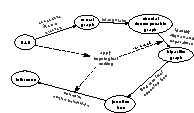
\includegraphics[width=0.9\textwidth]{img/jt_roadmap_nojust}%
	 }}
	 \only<2>{
	 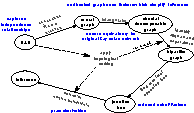
\includegraphics[width=0.9\textwidth]{img/jt_roadmap}%
	 }
	 \notesonly{
	 \caption{A road to efficient inference and a handwavy justification for the different steps}%
	 }
\end{figure}

\end{frame}

\subsection{Constructing Bayesian Networks}

\begin{frame} \frametitle{\subsubsecname}

	\begin{figure}[h]
		 \centering
		 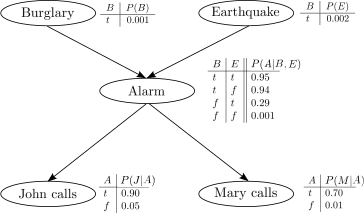
\includegraphics[width=0.5\textwidth]{img/section3_fig5_v2_2}%
		 \caption{DAG of the Californian example}
	\end{figure}
	
%	\only<2>{
%	\begin{itemize}
%		\item set of random variables 
%			$\leadsto$ nodes of the graph
%		\item direct influences between variables 
%			$\leadsto$ directed links between nodes
%		\item nodes $x_i$ are annotated with the conditional probabilities\\
%			\quad$P\big(X_i\,|\, \text{parents}(X_i)\big)$
%	\end{itemize}
%	} 
Considering statistical dependencies, only 10 instead of 31 entries have to be stored.
	{ \small
		\begin{align} 
			P(J,M,A,B,E) \stackrel{\substack{\text{product}\\\text{rule}}}{=}& 
			P(J|M,A,B,E) \, P(M|A,B,E) \, P(A|B,E) \, P(B|E) \, P(E) \\\slidesonly{\vspace{-5mm}}
			\stackrel{\substack{\text{cond.}\\\text{indep.}}}{=}& P(J|A) \, P(M|A) \, P(A|B,E) \, P(B) \, P(E)
		\end{align}
	}
\end{frame}

\begin{frame}\frametitle{\secname}
  
Bayesian Networks are a factorization of the full joint distribution\footnote{See Ch. 14 from \citep{russell2016artificial} for more details.}:

\begin{equation}
P(X_{1},\ldots,X_{n}) = \prod_{i=1}^{n} P(X_{i} | parents(X_{i}))
\end{equation}
    
\begin{itemize}
\item We only need to condition on the direct parents of any node $X_i$

\pause 
\item The factorization enables us to construct the \emph{directed acyclic graph} (DAG).
\item We can also use the DAG to formulate the factorization.
\end{itemize}

\begin{equation}
\mathit{DAG}_{\text{Bayes.Net}} \quad \corresponds \quad \prod_{i=1}^{n} P(X_{i} | parents(X_{i}))
\end{equation}
    
\end{frame}

\subsection{The Junction tree algorithm}

\begin{frame}\frametitle{\subsecname}

We need a representation that scales well for large DAGs to perform marginalisation (``summing out'') and conditioning more efficiently.

The Junction tree algorithm converts into a tree structure made up of \emph{cliques} and \emph{separators}.

\question{What is a difference between a DAG and a tree?}

\pause

- A tree structure guarantees that the path between any two nodes is unique.

\end{frame}

\begin{frame} \frametitle{Trees}
	\begin{itemize}
	\item\textbf{tree}: graph where each existing path 
			between nodes is \emph{unique}
	
	\vspace{2mm}
	\begin{center}
	\begin{tabular}{cc}
		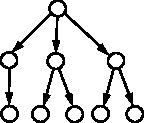
\includegraphics[width=4cm]{img/tree_directed}
		&
		\hspace{-5mm}
		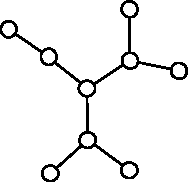
\includegraphics[width=5cm]{img/tree_undirected} \\
		directed tree & \hspace{-5mm} undirected tree 
	\end{tabular}
	\end{center}
	\end{itemize}
\end{frame}

\subsection{Decomposable Undirected Graphs}

\mode<presentation>{
\begin{frame} 
    \begin{center} \huge
        \subsecname
    \end{center}
    \begin{figure}[h]
	 \centering
	 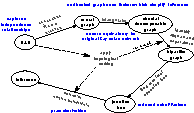
\includegraphics[width=0.8\textwidth]{img/jt_roadmap}%
	\end{figure}
    %\begin{center}   
		%\begin{align*}
		%\text{DAG}
		%\longrightarrow \substack{\text{moral}\\\text{graph}}
		%\longrightarrow \substack{\text{\textcolor{blue}{decomposable}}\\\text{\textcolor{blue}{graph}}}
		%\longrightarrow \substack{\text{bipartite}\\\text{graph}}
		%\longrightarrow \substack{\text{Junction}\\\text{Tree}}
		%\end{align*}
    %\end{center}
\end{frame}
}

% -----------------------------------------------------------------------------
\begin{frame} \frametitle{Undirected Graph}
\begin{figure}
	\centering
	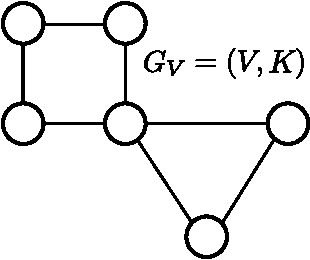
\includegraphics[width=4cm]{img/section3_fig9}
	 \caption{undirected graph \ensuremath{G_V} with vertices \ensuremath{V} and edges \ensuremath{K}} 
\end{figure}
\end{frame}

\mode<article>{
Separate $G$ (undirected graph) into two separate subgraphs $G_A$ and $G_B$
,
such that node $C$ lies on the path between \underline{any} node in $G_A$ and \underline{any} other node in $G_B$. 

\textbf{Remark}:
$C$ can also be a set of nodes (cf. ).
}

\subsubsection{Cliques and separators}

% -----------------------------------------------------------------------------
\begin{frame} \frametitle{Separators}

\only<1>{
\mode<presentation>{
	\begin{figure}
	\centering
	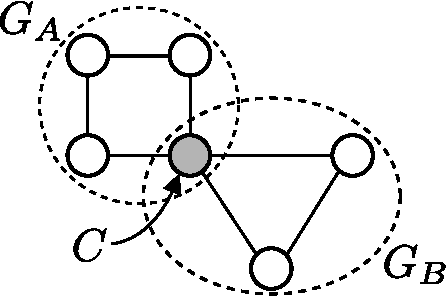
\includegraphics[width=5cm]{img/section3_fig10}
	\notesonly{\caption}\slidesonly{\caption*}{node C separates subsets A and B} 
	\end{figure}
}
}
\only<2>{
\begin{figure}[h]
     \centering
     \savebox{\imagebox}{
	 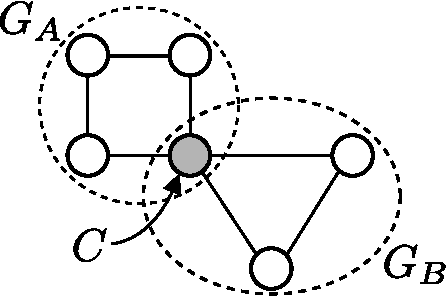
\includegraphics[width=0.4\textwidth]{img/section3_fig10}}%
     \begin{subfigure}[t]{0.35\textwidth}
         \centering
         \usebox{\imagebox}% Place largest image
         \caption{node C}
         \label{fig:nodes}
     \end{subfigure}
     \hspace{3mm}
     \begin{subfigure}[t]{0.4\textwidth}
         \centering
         \raisebox{\dimexpr.5\ht\imagebox-.5\height}{% Raise smaller image into place
         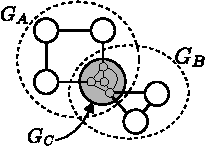
\includegraphics[width=0.95\textwidth]{img/section3_fig10_cset}
         }
         \caption{set of nodes C}
         \label{fig:setc}
     \end{subfigure}
     \caption{subgraphs A and B separated by C}
	 \label{fig:regression}
\end{figure}
}
	\slidesonly{\vspace{-2mm}}
	\begin{block}{Separator}
		A set $C$ of nodes \textbf{separates} two undirected subgraphs $G_A$ and $G_B$ 
		if \emph{every} path from node set $A$ to node set $B$ 
		has to pass through an element of $C$.
	\end{block}
\end{frame}

\subsubsection{Decomposable graphs}

% -----------------------------------------------------------------------------
\begin{frame}{Only} \frametitle{\subsubsecname}
	\vspace{-2mm}
	\begingroup
	\slidesonly{\footnotesize}
	\begin{itemize}
		\item $A,B,C$ are a \textbf{proper decomposition} 
			of an undirected graph $G = (V,K)$ if:
	%\slidesonly{\vspace{-4mm}}
			\begin{itemize}
				\item $A,B,C$ are non-empty and 
					disjoint subsets with $V=A \cup B \cup C$,
				\item $C$ separates $G_A$ and $G_B$, and
				\item subgraph $G_C$ is complete.
			\end{itemize}
		\item $G$ is \textbf{decomposable} if it is complete, 
			or a proper decomposition $A,B,C$ exist,
			\underline{where} $G_{A\cup C}$ and $G_{B \cup C}$ are decomposable.
	\end{itemize}
	\endgroup
	
	\slidesonly{\vspace{-4mm}}
	
	\pause
	
	\question{Are the following (i) a proper decomposition, (ii) decomposable graphs? \notesonly{(cf. \figref{fig:decompex1}, \figref{fig:decompex2}, \figref{fig:propernotdecompexample} and \figref{fig:propernotdecompexample4})} }

	\slidesonly{\vspace{-9mm}}
	
	\begin{enumerate}
	\item<only@2,3>[]
		%\begin{figure}[h]
		\begin{center}
		%\centering
		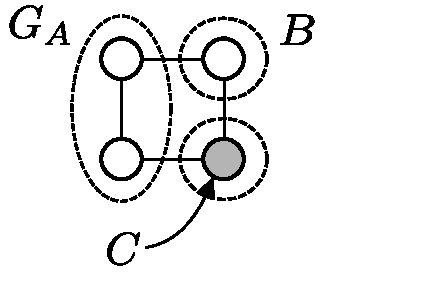
\includegraphics[width=5cm]{img/section3_fig10_sub}
		\only<3>{\captionof{figure}{not a proper decomposition \notesonly{\\}and not decomposable}
		}
		\label{fig:decompex1}
		\end{center}
	\item<only@4,5>[]
		%\begin{figure}[h]
		%\centering
		\begin{center}
		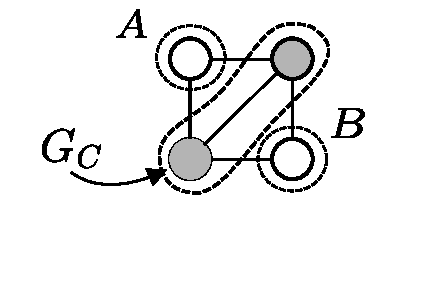
\includegraphics[width=5cm]{img/section3_fig10_sub_2}
		\only<5>{\captionof{figure}{a proper decomposition\notesonly{\\} and decomposable}
		}
		\label{fig:decompex2}
		%\end{figure}
		\end{center}
	\item<only@6,7>[]
	
		\begin{figure}[h]
		 \centering
		 \savebox{\imagebox}{
		 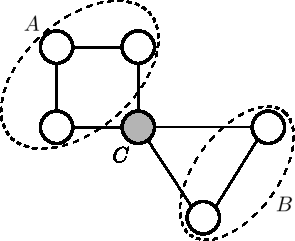
\includegraphics[width=0.3\textwidth]{img/section3_fig12}}%
		 \begin{subfigure}[t]{0.35\textwidth}
			 \centering
			 \usebox{\imagebox}% Place largest image
			 \caption{example decomposition}
			 \label{fig:propernotdecompgraph}
		 \end{subfigure}
		 \hspace{7mm}
		 \begin{subfigure}[t]{0.3\textwidth}
			 \centering
			 \raisebox{\dimexpr.5\ht\imagebox-.5\height}{% Raise smaller image into place
			 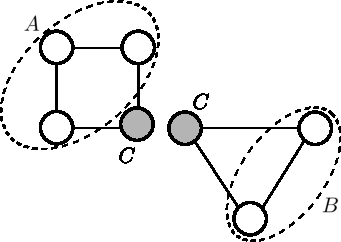
\includegraphics[width=0.99\textwidth]{img/section3_fig12_v2}
			 }
			 \caption{\underline{Hint}
			 \only<7>{: because $G_{A \cup C}$ is not decomposable}
			 }
			 \label{fig:hintnotdecomp}
		 \end{subfigure}
		 \only<7>{\caption{a proper decomposition but not decomposable}}
		 \label{fig:propernotdecompexample}
		\end{figure}
	
	\item<only@8,9>[]
	
		\begin{figure}[h]
		 \centering
		 \savebox{\imagebox}{
		 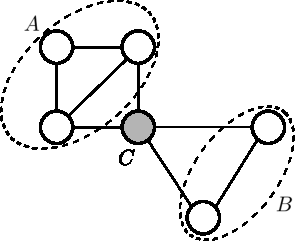
\includegraphics[width=0.3\textwidth]{img/section3_fig13}}%
		 \begin{subfigure}[t]{0.35\textwidth}
			 \centering
			 \usebox{\imagebox}% Place largest image
			 \caption{example decomposition}
			 \label{fig:propernotdecompgraph}
		 \end{subfigure}
		 \hspace{7mm}
		 \begin{subfigure}[t]{0.3\textwidth}
			 \centering
			 \raisebox{\dimexpr.5\ht\imagebox-.5\height}{% Raise smaller image into place
			 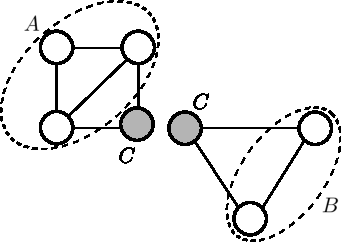
\includegraphics[width=0.99\textwidth]{img/section3_fig13_v2}
			 }
			 \caption{\underline{Hint}
			 \only<9>{: because $G_{A \cup C}$ is decomposable and $G_{A \cup B}$ is complete}
			 }
			 \label{fig:hintnotdecomp}
		 \end{subfigure}
		 \only<9>{\caption{a proper decomposition and decomposable}}
		 \label{fig:propernotdecompexample4}
		\end{figure}
	
	\end{enumerate}
	
\end{frame}

\begin{frame}\frametitle{\subsubsecname}

	\question{Why are we interested in decomposable graphs?}\\
	
	
	\pause	
	
	\slidesonly{\vspace{-10mm}}
	
	%\begin{figure}[h]
	%\centering
	%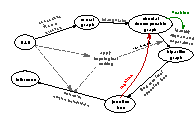
\includegraphics[height=5cm]{img/jt_roadmap_requirement}
	%\notesonly{\caption{The construction of a junction tree requires a decomposable graph of cliques.}}
	%\end{figure}
	
	\begin{figure}[h]
		 \centering
		 \hspace{-10mm}
		 \savebox{\imagebox}{
		 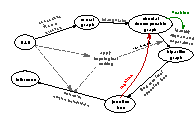
\includegraphics[width=0.5\textwidth]{img/jt_roadmap_requirement}}%
		 \begin{subfigure}[t]{0.3\textwidth}
			 \centering
			 \usebox{\imagebox}% Place largest image
		 \end{subfigure}
		 \hspace{15mm}
		 \begin{subfigure}[t]{0.35\textwidth}
			 \centering
			 \raisebox{\dimexpr.5\ht\imagebox-.5\height}{% Raise smaller image into place
			 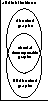
\includegraphics[width=0.3\textwidth]{img/directed_chordal_undirected_vertical}
			 }
		 \end{subfigure}
		 \mode<article>{\caption{The construction of a junction tree requires a decomposable graph of cliques.}
		 }
		\end{figure}
	
	\slidesonly{\vspace{-5mm}}
	
	
	- The short answer\notesonly{\footnote{Not required but if interested in more formal justifications see Ch 3.4 and Ch 4 from \citep{koller2009probabilistic}}}:
	\begin{enumerate}[(a)]
	\item it is a requirement for the construction of junction trees \notesonly{(cf. \sectionref{sec:constructjt})}
	\item decomposable graphs allow us to form a \emph{bipartite graph} of cliques and separators.
	\end{enumerate}
	
\end{frame}

\newpage

% -----------------------------------------------------------------------------
\begin{frame} \frametitle{\secname}

	\begin{block}{Cliques and separators}
	\begin{itemize}
		\item \textbf{cliques} are \underline{maximally complete subgraphs}
		\item decomposable graphs can be decomposed into cliques and separators
		\item cliques and separators form a \emph{bipartite graph} (cf. \figref{fig:cliquessepformbipartite})
	\end{itemize}
	\end{block}
	
	\slidesonly{\vspace{4mm}}
	
	%\begin{figure}[h]
	{
	\centering
	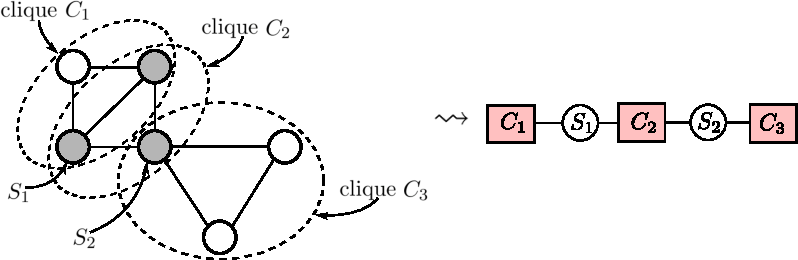
\includegraphics[height=3.5cm]{img/section3_fig15}
	\captionof{figure}{a decomposable graph and corresponding bipartite graph}
	\label{fig:cliquessepformbipartite}
	%\end{figure
	}
	
		
\end{frame}


\begin{frame}\frametitle{\subsubsecname}

\only<1>{
\mode<presentation>{
		\begin{figure}[h]
		 \centering
		 \savebox{\imagebox}{
		 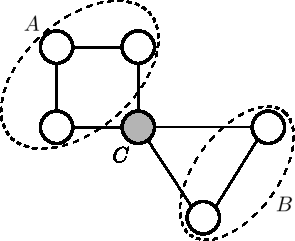
\includegraphics[width=0.3\textwidth]{img/section3_fig12}}%
		 \begin{subfigure}[t]{0.35\textwidth}
			 \centering
			 \usebox{\imagebox}% Place largest image
			 \caption{example decomposition}
		 \end{subfigure}
		 \hspace{7mm}
		 \begin{subfigure}[t]{0.3\textwidth}
			 \centering
			 \raisebox{\dimexpr.5\ht\imagebox-.5\height}{% Raise smaller image into place
			 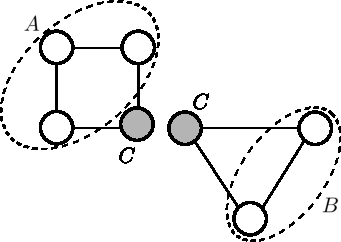
\includegraphics[width=0.99\textwidth]{img/section3_fig12_v2}
			 }
			 \caption{because $G_{A \cup C}$ is not decomposable}
		 \end{subfigure}
		 \caption{a proper decomposition but not decomposable}
		\end{figure}
}
}
	

	\question{What if we don't have a decomposable graph \notesonly{as in \figref{fig:propernotdecompexample}}?}\\
	
	\pause 
	
	- We apply triangulation. We add a \emph{chord}, i.e. ``shortcut'' edges to eliminate any ``circles'' (i.e. cycles) of 4+ vertices.
	
	\pause 
	
	According to Ch 9.4.3 in \citep{koller2009probabilistic}, constructing the \emph{chordal graph} is actually a heuristic of elimination ordering. It plays a role in keeping the size of cliques small. Smaller cliques allow for a more ``modular'' bipartite graph which leads to faster computation during inference.
	
\end{frame}


\mode*

\clearpage

\mode<all>
\subsubsection{Triangulation}

\begin{frame}\frametitle{Cycles and chords}

\slidesonly{\vspace{-3mm}}

\begin{figure}[h]
\centering
	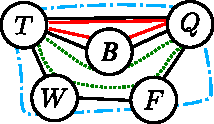
\includegraphics[height=2.cm]{img/cycles2}
	\mode<article>{
	\caption{Identifying cycles in an undirected graph}
	}
\end{figure}

\slidesonly{\vspace{-3mm}}

\begin{itemize}
\item \emph{Cycle}: A closed path with \textbf{no} repeated vertices \slidesonly{except}\notesonly{other than} $V_{\text{start}}=V_{\text{end}}$.
\item \emph{Chords}: Given a cycle, an edge is a chord if it connects two nodes that are non-adjacent on the cycle.
\item \emph{Chordless} cycle: \textbf{All} two \textbf{non}-adjacent vertices on the cycle are \textbf{not} joined by any edge.
\item \emph{Triangulated graph} ($\corresponds$ \emph{Chordal graph}): A graph \textbf{without} chordless cycles of 4+ vertices.\notesonly{\footnote{cf: Definition 2.24 on Ch. 2.2.4 in \citep{koller2009probabilistic}
%\citep{Jebaraslides}
}
}
\begin{flushright}
{\footnotesize(too many double negatives!!!)}
\end{flushright}
\end{itemize}

\slidesonly{\vspace{-2mm}}

\begin{block}{Triangulation}
Construct a chordal graph by adding \emph{chords} (``shortcut'' edges) to all cycles of length 4+.
\end{block} 

\end{frame}

%\newpage

\subsubsection{Triangulation: Examples}

\begin{frame}{Only} \frametitle{\subsubsecname}

\mode<presentation>{
\begin{block}{Triangulation}
Construct a chordal graph by adding \emph{chords} (``shortcut'' edges) all cycles of length 4+.
\end{block} 
}

\begin{enumerate}
\item<only@1>[]

	Consider the following graph with vertices $A,B,C,E$ \notesonly{in \figref{fig:triangulateexample1} }and add chords where necessary:
	\slidesonly{\textbf{(see blackboard)}}


	\begin{figure}[h]
	\centering
	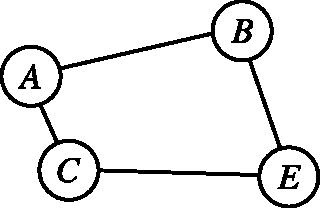
\includegraphics[height=2.5cm]{img/graph_example_triangulate}
	\caption{a non-decomposable graph}
	\label{fig:triangulateexample1}
	\end{figure}

\mode<article>{
		\begin{figure}[h]
		 \centering
		 \savebox{\imagebox}{
		 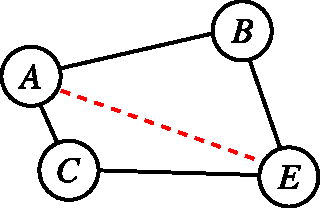
\includegraphics[width=0.2\textwidth]{img/graph_example_triangulate_sol1}}%
		 \begin{subfigure}[t]{0.25\textwidth}
			 \centering
			 \usebox{\imagebox}% Place largest image
			 %\caption{...}
		 \end{subfigure}
		 \hspace{7mm}
		 \begin{subfigure}[t]{0.2\textwidth}
			 \centering
			 \raisebox{\dimexpr.5\ht\imagebox-.5\height}{% Raise smaller image into place
			 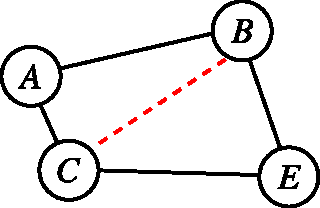
\includegraphics[width=0.99\textwidth]{img/graph_example_triangulate_sol2}
			 }
			 %\caption{...}%
		 \end{subfigure}
		 \caption{Possible triangulations for graph in \figref{fig:triangulateexample1}}
		\end{figure}
}


\item<only@2,3>[]

	Consider the following graph with vertices $A,B,C,W,E,F$ \notesonly{in \figref{fig:triangulateexample2} } and add chords where necessary:\\
	\slidesonly{\textbf{(see blackboard)}}


		\begin{figure}[h]
		 \centering
		 \savebox{\imagebox}{
		 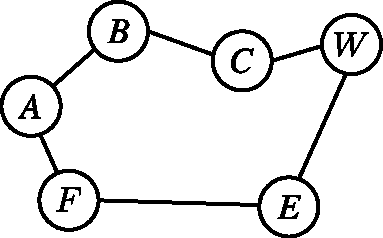
\includegraphics[width=0.25\textwidth]{img/graph_example2_triangulate}}%
		 \begin{subfigure}[t]{0.25\textwidth}
			 \centering
			 \usebox{\imagebox}% Place largest image
			 \caption{example graph to triangulate}
		 \end{subfigure}
		 \hspace{7mm}
		 \visible<3>{
		 \begin{subfigure}[t]{0.25\textwidth}
			 \centering
			 \raisebox{\dimexpr.5\ht\imagebox-.5\height}{% Raise smaller image into place
			 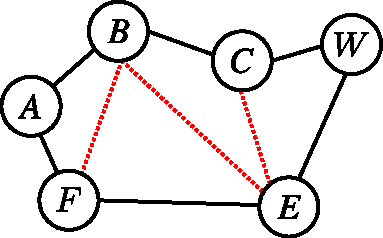
\includegraphics[width=0.99\textwidth]{img/graph_example2_triangulate_sol1}
			 }
			 \caption{One possible and non-unique triangulation}%
		 \end{subfigure}
		 \caption{Triangulation example}
		 \label{fig:triangulateexample2}
		 }
		\end{figure}

\item<only@4,5>[]

	\question{Is this a chordal graph\notesonly{ (c.f. \figref{fig:triangulateexample3})}? i.e. does it contain chordless cycles with 4+ vertices?}\\


		\begin{figure}[h]
		 \centering
		 \savebox{\imagebox}{
		 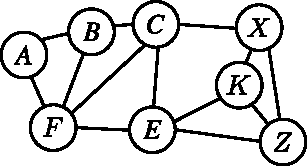
\includegraphics[width=0.3\textwidth]{img/graph_example3_triangulate}}%
		 \begin{subfigure}[t]{0.35\textwidth}
			 \centering
			 \usebox{\imagebox}% Place largest image
			 \caption{example graph}
		 \end{subfigure}
		 \hspace{5mm}
		 \visible<5>{
		 \begin{subfigure}[t]{0.3\textwidth}
			 \centering
			 \raisebox{\dimexpr.5\ht\imagebox-.5\height}{% Raise smaller image into place
			 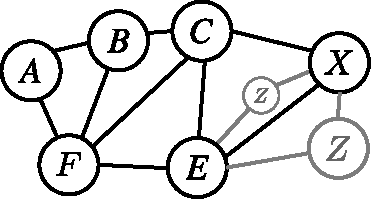
\includegraphics[width=0.99\textwidth]{img/graph_example3_triangulate_HINT}
			 }
		 \mode<article>{
			 \caption{The cycles CEKX and CEZX both require chords for the graph to be chordal.}%
			 }
		 \end{subfigure}
		 \mode<article>{
		 \caption{Determining if a graph is chordal}%
		 }
		 \label{fig:triangulateexample3}
		 }
		\end{figure}
		
\end{enumerate}

\end{frame}

\mode*

\clearpage
\newpage

\mode<all>
% =============================================================================
\subsection{Construction of the Junction Tree}\label{sec:constructjt}

\begin{frame} 
\mode<presentation>{
    \begin{center} \huge
        \secname
    \end{center}
    \begin{figure}[h]
	 \centering
	 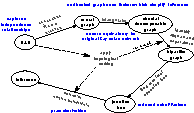
\includegraphics[width=0.8\textwidth]{img/jt_roadmap}%
	\end{figure}
}
\end{frame}

\subsubsection{The running intersection property}

\begin{frame}\frametitle{\subsubsecname}
 
    \begin{minipage}{0.5\textwidth}
        \begin{block}{The running intersection property}
            %\small
            All nodes on the path between two 
            cliques, which both contain variable $X$, 
            also contain $X$.
        \end{block} 
    \end{minipage}
    \mode<presentation>{
    \hfill
    \begin{minipage}{0.4\textwidth}
            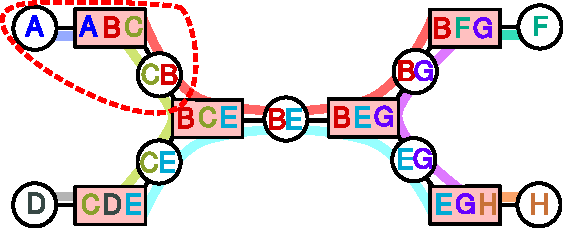
\includegraphics[width=5cm]{img/junction_tree_bipartite}
            \mode<article>{
            \captionof{figure}{The running intersection property}
            }
    \end{minipage}
    }
    \mode<article>{
    
        %\begin{figure}[h]
        {
            \centering
            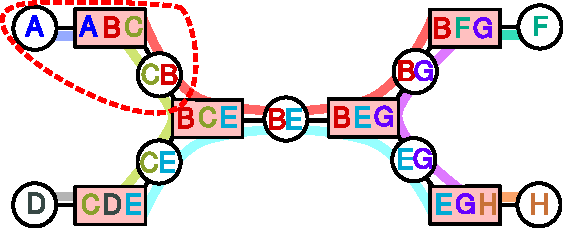
\includegraphics[width=6cm]{img/junction_tree_bipartite}
            \captionof{figure}{The running intersection property}
        }
        %\end{figure}
    }

\only<2>{


\question{Is the following a valid junction tree? \notesonly{ (cf. \figref{fig:isvalidjtexample1})}}\\

        %\begin{figure}[h]
        {
            \centering 
            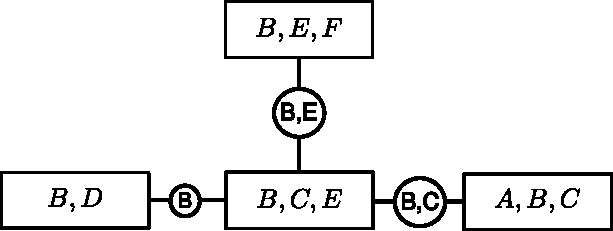
\includegraphics[width=5cm]{img/graph_example_isvalid_junction_tree}
            \mode<article>{
            \captionof{figure}{A valid junction tree}
            }
            \label{fig:isvalidjtexample1}
        }%\end{figure}
}

\only<3,4>{
\question{Which of the following remains a valid junction tree? (irrespective of being useful for exact inference)
 \notesonly{ (cf. \figref{fig:isvalidjtexample2} and \figref{fig:isvalidjtexample3})}}
}

\only<3>{

        %\begin{figure}[h]
        {
            \centering 
            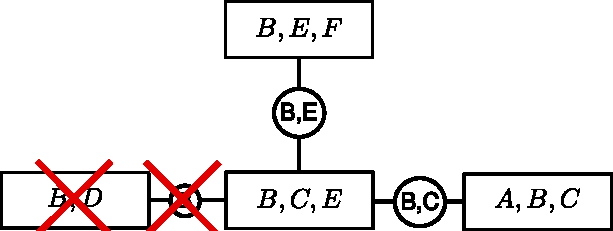
\includegraphics[width=5cm]{img/graph_example_isvalid2_junction_tree}
            \mode<article>{
            \captionof{figure}{This graph remains a valid junction tree}
            }
            \label{fig:isvalidjtexample2}
            }
        %\end{figure}
}
\only<4>{
        %\begin{figure}[h]
        {
            \centering 
            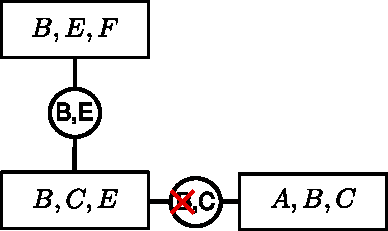
\includegraphics[width=5cm]{img/graph_example_isvalid3_junction_tree}
            \mode<article>{
            \captionof{figure}{This graph no longer qualifies as a junction tree}
            \label{fig:isvalidjtexample3}
            }
            }
        %\end{figure}
}

\end{frame}

\subsection{Identify cliques and separators to form a bipartite graph}

% -----------------------------------------------------------------------------
\begin{frame} \frametitle{\subsecname
}
					\slidesonly{\vspace{5mm}}
				\begin{itemize}
					\item cliques are \underline{maximally} complete subgraphs\\
					(sub-cliques are automatically absorbed)
					\item cliques can be found by elimination \\
					
					\slidesonly{\vspace{10mm}}
					\textbf{Caution: only eliminate a node if it is not part of another clique}
					\slidesonly{\vspace{5mm}}
					%\item sub-cliques $\{A,B\} \subseteq \{A,B,C\}$ are absorbed
					\item requires variable ordering by topological sorting: 
						F, D, E, C, B, A
				\end{itemize}
	
	\mode<presentation>{
	\begin{textblock}{}(12,2.5)
		\includegraphics<1->[width=3.cm]{img/graph_example_dag_highlight}
		%\includegraphics<2->[width=3.cm]{img/graph_example_cliques_chordal.jpg}
	\end{textblock}
	}
	
	\mode<article>{
		\begin{figure}[h]
		\centering
		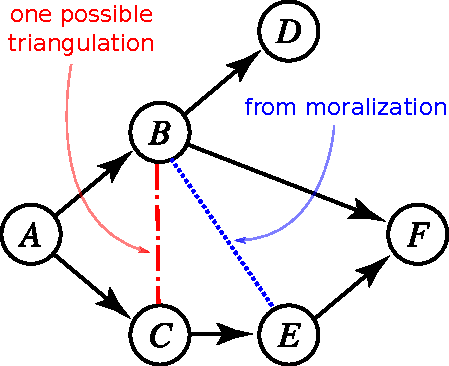
\includegraphics[height=3.5cm]{img/graph_example_dag_highlight}
		\mode<article>{\caption{Example graph from the lecture.}}
		\label{fig:lecexamplecdecompgraph}
		\end{figure}
	}
	
	
	%\begin{textblock}{15}(.5,8.5)
		%\begin{center}
		%\includegraphics<1>[height=3.5cm]{img/graph_example_dag.jpg}
		%\includegraphics<2>[height=3.5cm]{img/graph_example_amoral}
		%\only<2>{\hspace{1cm}}
		%\includegraphics<2>[height=3.5cm]{img/graph_example_moral.png}
		%\includegraphics<3>[height=3.5cm]{img/graph_example_chordal}
		%\only<3>{\hspace{1cm}}
		%\includegraphics<3>[height=3.5cm]{img/graph_example_chordal2}
		%\only<4>{\vspace{7mm}}
		\begin{figure}[h]
		\centering
		\includegraphics<2>[height=2.5cm]{img/graph_example_clique_elimination}
		\mode<article>{
		\caption{Identifying cliques by elimination}
		}
		\end{figure}
		%\includegraphics<3>[height=3.5cm]{img/graph_example_clique_graph}
		%\includegraphics<6>[height=3.5cm]{img/graph_example_junction_tree_v2}
		%\end{center}
	%\end{textblock}
\end{frame}

\subsection{From bipartite graph to junction tree}

\begin{frame} \frametitle{\subsecname
}
		\begin{itemize}		
			\item construct bipartite graph: 
				\only<1>{ \begin{itemize}
					\item edges weighted by separator size 
						$\rightarrow$ number of nodes within separator
					\item find a {\em maximal spanning tree} 
				\end{itemize}}	
			\item<2-> junction tree for inference
				\only<2>{ \begin{itemize}
					\item maximal spanning tree of the clique graph
					\item data structure for \\ belief propagation
					\item not always unique
				\end{itemize}}			
		\end{itemize}
	
	\mode<presentation>{
	\begin{textblock}{}(12,2.5)
		\includegraphics<1->[width=3cm]{img/graph_example_cliques_chordal.jpg}
	\end{textblock}
	}
	\mode<article>{
		\begin{center}
		%\begin{figure}[h]
		%\centering
		\includegraphics<1>[height=3.5cm]{img/graph_example_cliques_chordal.jpg}
		\mode<article>{\captionof{figure}{Idnetification of cliques and separators in example graph form \figref{fig:lecexamplecdecompgraph}}}
		\label{fig:lecexamplecliques}
		%\end{figure}
		\end{center}
	}
	
		\begin{center}
		%\begin{figure}[h]
		%\centering
		\includegraphics<1>[height=3.5cm]{img/graph_example_clique_graph}
		\mode<article>{\captionof{figure}{bipartite graph for \figref{fig:lecexamplecliques}}}
		\label{fig:lecbipartitegraph}
		%\end{figure}
		\end{center}
		
		\begin{center}
		%\begin{figure}[h]
		%\centering
		\includegraphics<2>[height=3.5cm]{img/graph_example_junction_tree_v2}
		\mode<article>{\captionof{figure}{junction tree to bipartite graph in \figref{fig:lecbipartitegraph}}}
		%\end{figure}
		\end{center}
		
\end{frame}

\subsection{Inference in a junction tree}

\begin{frame}\frametitle{\subsecname}

\begin{enumerate}
\item clique potentials (non-negative function) for each clique (get definitions from DAG)
\item order initialization according to topological sorting (parent $\rightarrow$ child)
\item add clique potential(s) for observed evidence(s)
\item perform message passing
\item extract marginals form messages
\item perform normalization
\end{enumerate}


\mode<presentation>{
	\begin{center}
		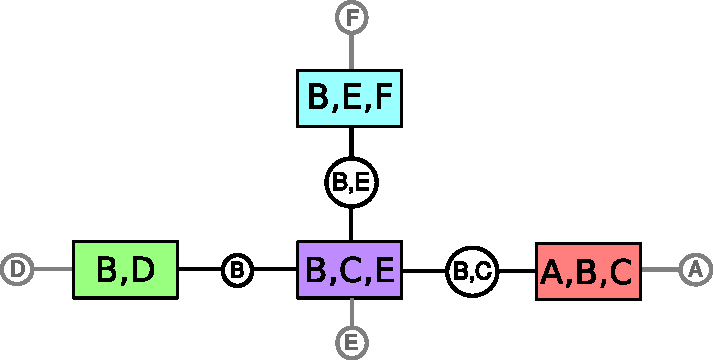
\includegraphics[height=3.5cm]{img/graph_example_junction_tree_v2}
	\end{center}
}

\end{frame}

\mode*

\clearpage

\mode<all>
\section{Message Passing}

\definecolor{darkgreen}{rgb}{0,0.6,0}

\mode<presentation>{
\begin{frame} 
    \begin{center} \huge
        \secname
    \end{center}
    \begin{center}
    a compact look-up-table
    \end{center}
\end{frame}
}

\subsection{Overview}

\begin{frame}\frametitle{Message Passing: Overview}

\begin{itemize}
\item essentially storage of local computations for faster look-up
\item will be used to calculate conditional probabilities in a junction tree by only using local ``simpler'' computations.
\item scales well with no. of variables.
\end{itemize}

\end{frame}

\subsection{Procedure}

% -----------------------------------------------------------------------------
\begin{frame} \frametitle{\secname: \subsecname}
	%\iitem{a third pass can calculate all other marginals}
	\begin{minipage}[c]{12.1cm}
		\begin{minipage}[][1cm][c]{8cm}
			\begin{itemize}
				\item first pass from root to leaves: \textcolor{red}{``request''}\\
				selecting the root (for tree structures any node can be the root, so not sensitive to choice of root node)
			\end{itemize}
		\end{minipage}
		\hfill \raisebox{-4mm}{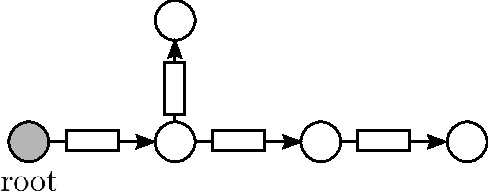
\includegraphics[width=4cm]{img/section3_fig20}} \\
		\begin{minipage}[c]{8cm}
			\begin{itemize}
				\item second pass from leaves to root: \textcolor{blue}{``collect''}\\
				collect messages from other neighbors
			\end{itemize}
		\end{minipage}
		\hfill \raisebox{-8mm}{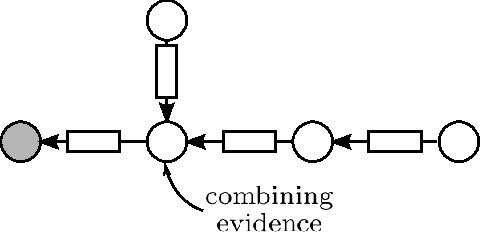
\includegraphics[width=4cm]{img/section3_fig21}} \\
		\pause
		\begin{minipage}{8cm}
			\begin{itemize}
				\item a third pass can calculate all other \\
					marginals: \textcolor{darkgreen}{``distribute''}\\
					third pass from root to leaves to compute the remaining messages.
			\end{itemize}
		\end{minipage}
		\hfill \raisebox{-6mm}{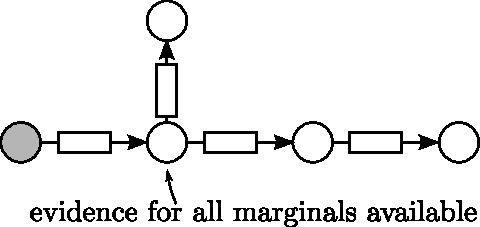
\includegraphics[width=4cm]{img/section3_fig22}} \\
	\end{minipage}
\end{frame}

\subsection{The sum-product algorithm}
% -----------------------------------------------------------------------------
\begin{frame} \frametitle{\subsecname}
	\vspace{-4mm}
	%\begin{minipage}{12cm}
		%\begin{minipage}{6.5cm}
			%\vspace{5mm}
			%\includegraphics[height=3.5cm]{img/tree_inference_product_message_v2}
			%\begin{itemize}
				%\item product message from $X_m$ to $f_s$
			%\end{itemize}
		%\end{minipage}
		%\hfill
		%\visible<2>{\begin{minipage}{6cm}
			%\hfill
			%\includegraphics[height=3.65cm]{img/tree_inference_sum_message_v2}
			%\vspace{2mm} 
			%\begin{itemize}
				%\item sum message from $f_s$ to $X_i$
			%\end{itemize}
		%\end{minipage}}
	%\end{minipage}
    
    Defining the messages between the different types of nodes in a bipartite graph (e.g. separators and cliques)\footnote{for details, see Ch. 8.4.4, p. 402 in \citep{bishop2006pattern}}

	%\hspace{-4mm}
	\begin{align}
		\mu_{X_m \to f_s}(X_m) &\;:=&&\kern-4ex
			\kern-3ex\prod_{l \in \text{neighbor}(X_m) \setminus\{f_s\}}\kern-3ex
			\mu_{f_l \to X_m}(X_m) \tag{product}\\[1mm] 
		\visible<2>{
		\mu_{f_s \to X_i}(X_i) &\;:=&&\kern-3ex 
			\sum_{X_m, \ldots, X_M}\kern-2ex f_s(X_i, X_m,\ldots, X_M) 
			\kern-5ex\prod_{k \in \text{neighbor}(f_s)\setminus\{X_i\}}\kern-5ex 
			\mu_{X_k \to f_s}(X_k) 
			\only<1>{\nonumber\hspace{10mm}}
			\only<2>{\tag{sum}}
		}
        \label{eq:sumproduct}
	\end{align}
	
	\mode<article>{
	\begin{itemize}
	\item The arguments of the messages follow the variables in the separator node.
	\item For the \emph{product} formula, the product runs over all clique potentials that are neighbors of the separator $X_m$, except for $f_s$ that the message is going to.
	\item For the \emph{sum} formula, the sum takes care of marginalizing over all the variables that are present in the outgoing clique potential $f_s$ but are absent from the variables inside the target separator. This is weighted by the product of messages that arrive at $f_s$ from other neighbors (i.e. we exclude the separator that the message is going to).
	\end{itemize}
	}
\end{frame}

\mode*

\clearpage

\mode<all>
\section{Message Passing}

\definecolor{darkgreen}{rgb}{0,0.6,0}


% -----------------------------------------------------------------------------
\begin{frame} \frametitle{Message passing}
	%\iitem{a third pass can calculate all other marginals}
	\begin{minipage}[c]{12.1cm}
		\begin{minipage}[][1cm][c]{8cm}
			\begin{itemize}
				\item first pass from root to leaves: ``request''
			\end{itemize}
		\end{minipage}
		\hfill \raisebox{-4mm}{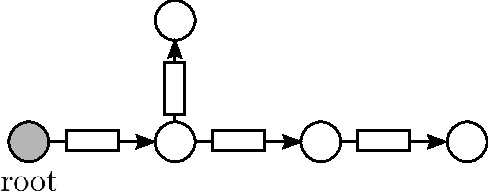
\includegraphics[width=4cm]{img/section3_fig20}} \\
		\begin{minipage}[c]{8cm}
			\begin{itemize}
				\item second pass from leaves to root: ``collect''
			\end{itemize}
		\end{minipage}
		\hfill \raisebox{-8mm}{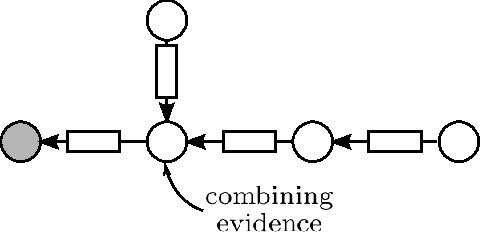
\includegraphics[width=4cm]{img/section3_fig21}} \\
		\pause
		\begin{minipage}{8cm}
			\begin{itemize}
				\item a third pass can calculate all other \\
					marginals: ``distribute''
					% third pass from root to leaves: ``distribute''
			\end{itemize}
		\end{minipage}
		\hfill \raisebox{-6mm}{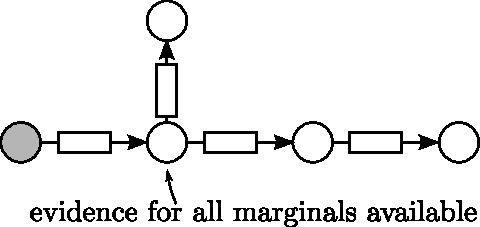
\includegraphics[width=4cm]{img/section3_fig22}} \\
	\end{minipage}
\end{frame}

\subsection{The sum-product algorithm}
% -----------------------------------------------------------------------------
\begin{frame} \frametitle{\subsecname}
	\vspace{-4mm}
	%\begin{minipage}{12cm}
		%\begin{minipage}{6.5cm}
			%\vspace{5mm}
			%\includegraphics[height=3.5cm]{img/tree_inference_product_message_v2}
			%\begin{itemize}
				%\item product message from $X_m$ to $f_s$
			%\end{itemize}
		%\end{minipage}
		%\hfill
		%\visible<2>{\begin{minipage}{6cm}
			%\hfill
			%\includegraphics[height=3.65cm]{img/tree_inference_sum_message_v2}
			%\vspace{2mm} 
			%\begin{itemize}
				%\item sum message from $f_s$ to $X_i$
			%\end{itemize}
		%\end{minipage}}
	%\end{minipage}
    
    Definining the messages between the different types of nodes in a bipartite graph (e.g. separators and cliques)\footnote{for details, see p. 402 in \citep{bishop2006pattern}}

	%\hspace{-4mm}
	\begin{align}
		\mu_{X_m \to f_s}(X_m) &\;:=&&\kern-4ex
			\kern-3ex\prod_{l \in \text{neighbor}(X_m) \setminus\{f_s\}}\kern-3ex
			\mu_{f_l \to X_m}(X_m) \tag{product}\\[1mm] 
		\visible<2>{
		\mu_{f_s \to X_i}(X_i) &\;:=&&\kern-3ex 
			\sum_{X_m, \ldots, X_M}\kern-2ex f_s(X_i, X_m,\ldots, X_M) 
			\kern-5ex\prod_{k \in \text{neighbor}(f_s)\setminus\{X_i\}}\kern-5ex 
			\mu_{X_k \to f_s}(X_k) 
			\only<1>{\nonumber\hspace{10mm}}
			\only<2>{\tag{sum}}
		}
        \label{eq:sumproduct}
	\end{align}
	
\end{frame}

\begin{frame} \frametitle{Inference}
	\begin{textblock}{14}(0.5,3)
	\begin{enumerate}
		\item<1-> initialization of the clique potentials $f_k(\mathcal X_k)$
			\only<1>{ \begin{itemize}
				\item in the order established by 
					topological sorting	\\(e.g.
					$A \to B \to C \to E \to D \to F$) \\[2mm]
					{\small\begin{tabular}{|c|c|c|c|}
					\hline 
					$f_1(A,B,C)$ & $f_2(B,C,E)$ & $f_3(B,D)$ & $f_4(B,E,F)$ \\
					\hline 
					%\hline
					%$P(A,B,C)$ & $\frac{P(B,C,E)}{P(B,C)}$ & $\frac{P(B,D)}{P(B)}$ 
					%	& $\frac{P(B,E,F)}{P(B,E)}$ \\
					%\hline
					$P(C|A)\,P(B|A)\,P(A)$ & $P(E|C)$ & $P(D|B)$ & $P(F|B,E)$ \\
					\hline
					\end{tabular} }
			\end{itemize} }
		\only<1>{\vspace{4mm}
			{\small $$ \hspace{-4mm} 
				P(A,B,C,D,E,F) \;\;=\;\; 
				P(A) \, P(B|A) \, P(C|A) \, P(D|B) \, P(E|C) \, P(F|B,E) 
			$$}
		}
		\item<2-> modification of the clique potentials by the observed evidence
			\only<2>{\begin{itemize}
				\item for each observation $Y=y$ find {\em one} 
					$f_k$ with $Y \in \mathcal X_k$
				\item add a separator node 
					{\footnotesize $
						f_k(Y) = 
						\left\{\begin{array}{c} 
							1, \; Y=y \\[-1mm]
							0, \; Y \neq y 
						\end{array}\right.
					$}
				\item example: $D=d$ and $E=e$ 
			\end{itemize} }
		\vspace{2mm}
		\item<3-> message passing 
			\only<3>{\begin{itemize}
				\item begin {\color{red}``request'' pass} 
					from arbitrary node $N$, e.g.~$A$
				\item wait for all message of {\color{blue}``collect'' pass} 
							to return
				\item send last {\color{darkgreen}``distribute'' pass} from $N$
				\itR  all marginals are computed simultaneously
			\end{itemize}}
		\vspace{2mm}
		\item<4-> calculate marginals from messages
			\only<4>{ \small
				$$
					P(C, \,D = d, E = e) 
						\quad=\quad \sum_{B}{} \;
							{\color{blue}\mu_{f_1 \to BC}(B,C)} \cdot 
							{\color{darkgreen} \mu_{f_2 \to BC}(B,C)} 
				$$
			}
		\item<5-> normalization yields conditional marginals
			\only<5>{ \small
				$$
					P(C\, | D = d, E = e) = \alpha \, \underbrace{P(C, \,D = d, E = e)}_{\tilde P(C)}, \quad\qquad\qquad \alpha = \frac{1}{\sum_C \tilde P(C)}
				$$ 
			}
	\end{enumerate}	
	\end{textblock}
	
	\begin{textblock}{15}(1.5,9.5)
		\begin{minipage}{12cm}
			\begin{minipage}{4cm}
				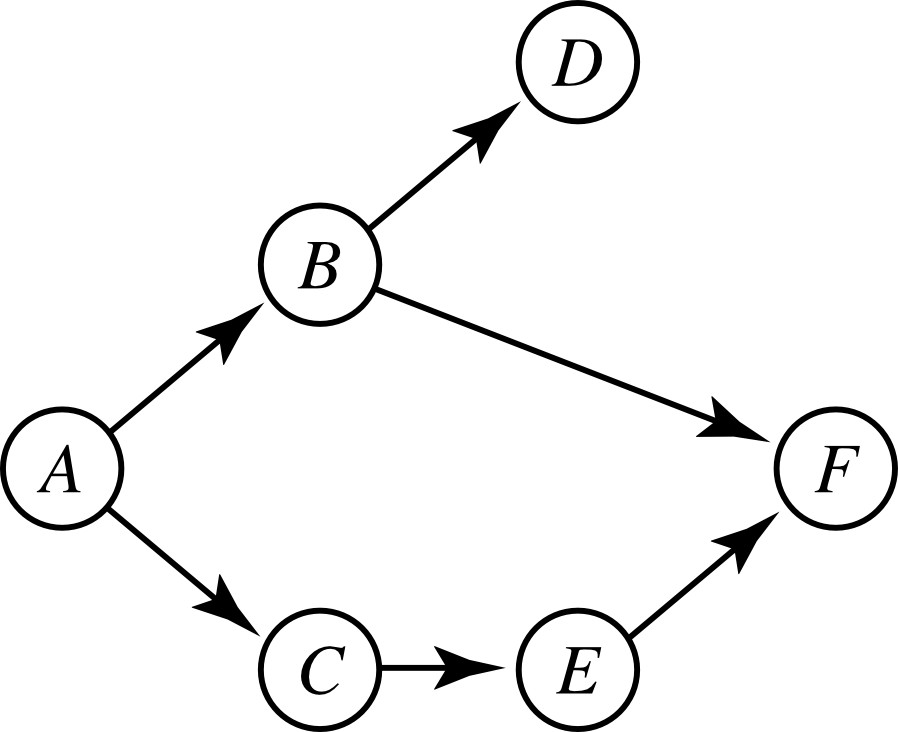
\includegraphics[width=3cm]{img/graph_example_dag.jpg}
			\end{minipage}
			\begin{minipage}{7cm}
				\includegraphics<1>[height=3cm]%
					{img/graph_example_junction_tree_init_v2.pdf}
				\includegraphics<2>[height=3.5cm]%
					{img/graph_example_junction_tree_evidence_v2.pdf}
				\includegraphics<3->[height=3.55cm]%
					{img/graph_example_junction_tree_messages_v2.pdf}
			\end{minipage}
		\end{minipage}
	\end{textblock}
\end{frame}

\begin{frame}{Only}

\mode<presentation>{

\placeimage{9.}{1}{img/graph_example_junction_tree_messages_v2_noextra}{height=2.5cm}

\begin{block}{sum-product}
\begingroup
\small
	\begin{align}
		\mu_{X_m \to f_s}(X_m) &\;:=&&\kern-4ex
			\kern-3ex\prod_{l \in \text{neighbor}(X_m) \setminus\{f_s\}}\kern-3ex
			\mu_{f_l \to X_m}(X_m) \tag{product}\\[1mm] 
		\mu_{f_s \to X_i}(X_i) &\;:=&&\kern-3ex 
			\sum_{X_m, \ldots, X_M}\kern-2ex f_s(X_i, X_m,\ldots, X_M) 
			\kern-5ex\prod_{k \in \text{neighbor}(f_s)\setminus\{X_i\}}\kern-5ex 
			\mu_{X_k \to f_s}(X_k) 
			\only<1>{\nonumber\hspace{10mm}}
			\only<2>{\tag{sum}}
	\end{align}
\endgroup
    \end{block}
    }
    
Define the messages by applying the sum-product-algorithm\notesonly{ from \eqref{eq:suproduct}}:

\begingroup
\footnotesize
\begin{enumerate}
 \item<only@1> Pick root (e.g. $f_{5}$), doesn't matter much%, no effect on the messages, but possibly affects the order in which we will define them   
 \item<only@1> assume we've done the request
 \item<only@1-> \textcolor{blue}{collect} (start at leaf node):
 \begin{itemize}
  \item<only@2> `branch on the right`:
  \begin{itemize}
  \item $\msg{f_{1}}{B,C}(B,C) := \sum_{A} f_{1}(A,B,C) \overbrace{\hcancel{\prod_{k \in \text{neigh.}(f_s)\setminus\{X_i\}}\kern-5ex 
			\mu_{X_k \to f_s}(X_k)}}^{\text{no other neighbors}}$
  \item $\msg{B,C}{f_{2}}(B,C) := \msg{f_{1}}{B,C}(B,C) = \sum_{A} f_{1}(A,B,C)$
  \end{itemize}
  \item<only@3> `top branch`:
  \begin{itemize}
  \item $\msg{f_{4}}{B,E}(B,E) := \sum_{F} f_{4}(B,E,F)$
  \item $\msg{B,E}{f_{2}}(B,E) := \msg{f_{4}}{B,E}(B,E) = \sum_{F} f_{4}(B,E,F)$
  \end{itemize}
  \item<only@4> `bottom branch`:
  \begin{itemize}
  \item $\msg{f_{6}}{E}(E) := f_{6}(E)$
  \item $\msg{E}{f_{2}}(E) := \msg{f_{6}}{E}(E) = f_{6}(E)$
  \end{itemize}
  \item<only@5> `left branch`:
  \begin{itemize}
  \item $\msg{f_{2}}{B}(B) := \sum_{B,E} f_{2}(B,C,E) \cdot \msg{E}{f_{2}}(E) \cdot \msg{B,E}{f_{2}}(B,E) \cdot \msg{B,E}{f_{2}}(B,E)$
  \item $\msg{B}{f_{3}}(B) := \msg{f_{2}}{B}(B)$
  \item $\msg{f_{3}}{D}(D) := \sum_{B} f_{3}(B,D) \cdot \msg{B}{f_{3}}(B)$
  \item $\msg{D}{f_{5}}(D) := \msg{f_{3}}{D}(D)$
  \end{itemize}
 \end{itemize}
\end{enumerate}
 \endgroup
\end{frame}

\subsubsection{The running intersection property}

\begin{frame}\frametitle{\subsubsecname}
 
    \begin{minipage}{0.4\textwidth}
        \begin{block}{The running intersection property}
            \small
            All nodes on the path between two 
            cliques, which both contain variable $X$, 
            also contain $X$.
        \end{block} 
    \end{minipage}
    \hfill
    \begin{minipage}{0.4\textwidth}
        %\begin{figure}[h]
            %\centering 
            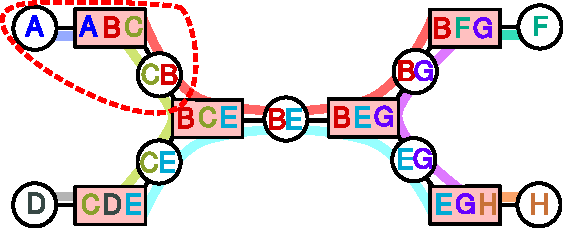
\includegraphics[width=5cm]{img/junction_tree_bipartite}
            \mode<article>{
            \captionof{figure}{The running intersection property}
            }
        %\end{figure}
    \end{minipage}

\only<2>{


\question{Is the following a valid junction tree?}

        \begin{figure}[h]
            \centering 
            \includegraphics[width=5cm]{img/graph_example_isvalid_junction_tree}
            \mode<article>{
            \caption{A valid junction tree}
            }
        \end{figure}
}

\only<3,4>{
\question{Which of the following remains a valid junction tree? (irrespective of being useful for exact inference)}
}

\only<3>{

        \begin{figure}[h]
            \centering 
            \includegraphics[width=5cm]{img/graph_example_isvalid2_junction_tree}
            \mode<article>{
            \caption{This graph remains a valid junction tree}
            }
        \end{figure}
}
\only<4>{
        \begin{figure}[h]
            \centering 
            \includegraphics[width=5cm]{img/graph_example_isvalid3_junction_tree}
            \mode<article>{
            \caption{This graph no longer qualifies as a junction tree}
            }
        \end{figure}
}

\end{frame}



\mode*

%\clearpage

\section{References}
\begin{frame}[allowframebreaks] \frametitle{References}
	\scriptsize
	\bibliographystyle{plainnat}
	\bibliography{bibliography}
\end{frame}

\end{rightcolumn}
\end{paracol}

\end{document}
